%                                                                 aa.dem
% AA vers. 9.1, LaTeX class for Astronomy & Astrophysics
% demonstration file
%                                                       (c) EDP Sciences
%-----------------------------------------------------------------------
%
% \documentclass[referee]{aa} % for a referee version
%\documentclass[onecolumn]{aa} % for a paper on 1 column  
%\documentclass[longauth]{aa} % for the long lists of affiliations 
%\documentclass[letter]{aa} % for the letters 
%\documentclass[bibyear]{aa} % if the references are not structured 
%                              according to the author-year natbib style

%

\documentclass{article}  

%
\usepackage{graphicx}
\usepackage{amsmath,amsfonts,amssymb}
\usepackage{natbib}



%%%%%%%%%%%%%%%%%%%%%%%%%%%%%%%%%%%%%%%%
\usepackage{txfonts}
\usepackage{xcolor}

\usepackage{blindtext}
%%%%%%%%%%%%%%%%%%%%%%%%%%%%%%%%%%%%%%%%
% \usepackage[options]{hyperref}
% To add links in your PDF file, use the package "hyperref"
% with options according to your LaTeX or PDFLaTeX drivers.
\usepackage{float}
%\usepackage{stfloats}
\usepackage{dblfloatfix}
\usepackage{afterpage}
\usepackage{ifthen}
\usepackage[morefloats=12]{morefloats}

\usepackage{placeins}
\usepackage{multicol}
%\usepackage[breaklinks,colorlinks,citecolor=blue]{hyperref}
\bibpunct{(}{)}{;}{a}{}{,}
\usepackage[switch]{lineno}
\definecolor{linkcolor}{rgb}{0.6,0,0}
\definecolor{citecolor}{rgb}{0,0,0.75}
\definecolor{urlcolor}{rgb}{0.12,0.46,0.7}
\usepackage[breaklinks, colorlinks, urlcolor=urlcolor,
    linkcolor=linkcolor,citecolor=citecolor,pdfencoding=auto]{hyperref}
\hypersetup{linktocpage}
\usepackage{bold-extra}

\usepackage{subcaption} % for subfigures
% new command for to dos
\newcommand{\todo}[1]{\textcolor{red}{\textbf{TODO:} #1}}

%Planck style file, to be used with A&A style to produce Planck papers for publication.
%
% version 28 September 2010 --- useful macros --- CRL
% version 17 October 2010   --- first cut at important instrument values, from Daniele Mennella and
%                               Francois Bouchet, 13 October 2010 --- CRL
% version 18 October 2010   --- LFI FWHM changed to one value per feed, rather than M & S separately
%                               LFI FWHM uncertainties added for individual feeds.  Corrections made
%                               to LFI values. --- Andrea Zacchei
% version 24 October 2010   --- added to and corrected definitions.  No changes made to instrument
%                               quantities. --- CRL 
% version 31 October 2010   --- added definition of \muKHz. --- CRL
%
% version 15 November 2010  --- fixed conflict with aa.cls in definition of \endtable
%                               by naming the command below "\endPlancktable".  See section
%                               13.16 of the Style Guide.
%
% version 06 December 2010  --- Set up names with and without units.
%                               Add \allearlypapers command to ensure that all early papers are
%                               included in the reference list.
%                               Define macro for the name of the 4He JT cooler.
%
% version 07 December 2010  --- removed extraneous "planck2011-1.2" entry in \allearlypapers
%
% version 12 December 2010  --- added \endPlancktablewide command to set tablenotes to the full
%                               page width in the \begin{table*}...\end{table*} environment when
%                               the ``twocolumn'' option is specified in the \documentclass command.
%                               (It would be more elegant to extract the appropriate width from the
%                               aa.cls system at the time of execution, but that is buried more
%                               deeply in the system than I investigated.)
%
% version 05 January 2011   --- added unit \MJysr.  HFI performance values updated per FRB email
%                               01/05/2011 02:38-0800, and Brendan Crill email 01/05/2011 18:08 -0800.
%
% version 06 January 2011   --- changed \scriptscriptstyle primes to \scriptstyle, to better match the
%                               tx fonts used by A&A.
%
% version 07 January 2011   --- modified \allearlypapers to correspond with final early paper list.  
%                               Fixed 545 GHz center frequency.
%
% version 07 January 2011b  --- changed LFI white-noise sensitivity numbers to correct problem with units
%
% version 05 July 2011      --- added \Msol and \Lsol to get the symbols for solar mass and luminosity.
%                               Deleted previous definitions of \solar and \sol, which were equivalent
%                               to the new \Msol.
%
% version 16 August 2011    --- changed comments on \endPlancktable and \endPlancktablewide for clarity
%
% version 11 September 2011 --- changed definition of \tablenote to make footnote labels italic, as per A\&A
%
% version 26 April 2011     --- changed definition of \Planck to agree with what is said in the Style Guide (!)
%
% version 04 Dec 2013       --- included 2013 results references
%
% version 17 Jan 2014       --- included fix to bibtex file v4.3, i.e. \providecommand{\sorthelp}[1]{}
%
% version 26 Jul 2014       --- fixed incompatibility problem with aa.cls v8.0 and v8.2.  v8.2 should now be used
%                               for all Planck papers.
%                           --- fixed problem in definition of "\all2013resultspapers" that introduced a blanck
%                               into the reference to p06b.
%                           --- removed all the parameter definition stuff at the end.  We weren't using it, and
%                               it took up a lot of space.
%
% version 28 Jan 2015       --- added "\alltwentyfiftennresultspapers" and corrected "\all2013resultspapers" to
%                               "\all20thirteenresultspapers",
%
% Usage:  after the \documentclass[traditabstract]{aa} command in the La\TeX\ input file,
%         add this command:      \input Planck.tex


\def\setsymbol#1#2{\expandafter\def\csname #1\endcsname{#2}}
\def\getsymbol#1{\csname #1\endcsname}

%-----------------------------------------------------------------------
% Planck
%-----------------------------------------------------------------------
\def\Planck{\textit{Planck}}

%-----------------------------------------------------------------------
% The Planck Helium-4 JT cooler
%-----------------------------------------------------------------------
\def\HeJT{$^4$He-JT}

%-----------------------------------------------------------------------
% To include all Planck Early Results papers in the reference lists
%-----------------------------------------------------------------------
\def\allearlypapers{\nocite{planck2011-1.1, planck2011-1.3, planck2011-1.4, planck2011-1.5, planck2011-1.6, planck2011-1.7, planck2011-1.10, planck2011-1.10sup, planck2011-5.1a, planck2011-5.1b, planck2011-5.2a, planck2011-5.2b, planck2011-5.2c, planck2011-6.1, planck2011-6.2, planck2011-6.3a, planck2011-6.4a, planck2011-6.4b, planck2011-6.6, planck2011-7.0, planck2011-7.2, planck2011-7.3, planck2011-7.7a, planck2011-7.7b, planck2011-7.12, planck2011-7.13}}

%-----------------------------------------------------------------------
% To include all Planck 2013 Results papers in the reference lists
%-----------------------------------------------------------------------
\def\alltwentythirteenresultspapers{\nocite{planck2013-p01, planck2013-p02, planck2013-p02a, planck2013-p02d, planck2013-p02b, planck2013-p03, planck2013-p03c, planck2013-p03f, planck2013-p03d, planck2013-p03e, planck2013-p01a, planck2013-p06, planck2013-p03a, planck2013-pip88, planck2013-p08, planck2013-p11, planck2013-p12, planck2013-p13, planck2013-p14, planck2013-p15, planck2013-p05b, planck2013-p17, planck2013-p09, planck2013-p09a, planck2013-p20, planck2013-p19, planck2013-pipaberration, planck2013-p05, planck2013-p05a, planck2013-pip56, planck2013-p06b, planck2013-p01a}}

%-----------------------------------------------------------------------
% To include all Planck 2015 Results papers in the reference lists
%-----------------------------------------------------------------------
\def\alltwentyfifteenresultspapers{\nocite{planck2014-a01, planck2014-a03, planck2014-a04, planck2014-a05, planck2014-a06, planck2014-a07, planck2014-a08, planck2014-a09, planck2014-a11, planck2014-a12, planck2014-a13, planck2014-a14, planck2014-a15, planck2014-a16, planck2014-a17, planck2014-a18, planck2014-a19, planck2014-a20, planck2014-a22, planck2014-a24, planck2014-a26, planck2014-a28, planck2014-a29, planck2014-a30, planck2014-a31, planck2014-a35, planck2014-a36, planck2014-a37, planck2014-ES}}

%-----------------------------------------------------------------------
% Tables
%-----------------------------------------------------------------------
\newbox\tablebox    \newdimen\tablewidth
\def\leaderfil{\leaders\hbox to 5pt{\hss.\hss}\hfil}
%
% use the following definition of \endPlancktable for ApJ style notes to tables, set to the 
%         width of the table
% \def\endPlancktable{\tablewidth=\wd\tablebox 
%
% use the following definitions of \endPlancktable and \endPlancktablewide for A&A style notes 
% set to one-column  or full-page width, respectively
\def\endPlancktable{\tablewidth=\columnwidth 
    $$\hss\copy\tablebox\hss$$
    \vskip-\lastskip\vskip -2pt}
\def\endPlancktablewide{\tablewidth=\textwidth 
    $$\hss\copy\tablebox\hss$$
    \vskip-\lastskip\vskip -2pt}
\def\tablenote#1 #2\par{\begingroup \parindent=0.8em
    \abovedisplayshortskip=0pt\belowdisplayshortskip=0pt
    \noindent
    $$\hss\vbox{\hsize\tablewidth \hangindent=\parindent \hangafter=1 \noindent
    \hbox to \parindent{$^#1$\hss}\strut#2\strut\par}\hss$$
    \endgroup}
\def\doubleline{\vskip 3pt\hrule \vskip 1.5pt \hrule \vskip 5pt}

%-----------------------------------------------------------------------
% useful macros
%-----------------------------------------------------------------------
%
\def\L2{\ifmmode L_2\else $L_2$\fi}
%
\def\dtt{\Delta T/T}
\def\DeltaT{\ifmmode \Delta T\else $\Delta T$\fi}
\def\deltat{\ifmmode \Delta t\else $\Delta t$\fi}
\def\fknee{\ifmmode f_{\rm knee}\else $f_{\rm knee}$\fi}
\def\Fmax{\ifmmode F_{\rm max}\else $F_{\rm max}$\fi}
%
\def\solar{\ifmmode{\rm M}_{\mathord\odot}\else${\rm M}_{\mathord\odot}$\fi}
\def\Msolar{\ifmmode{\rm M}_{\mathord\odot}\else${\rm M}_{\mathord\odot}$\fi}
\def\Lsolar{\ifmmode{\rm L}_{\mathord\odot}\else${\rm L}_{\mathord\odot}$\fi}
%
\def\inv{\ifmmode^{-1}\else$^{-1}$\fi}
\def\mo{\ifmmode^{-1}\else$^{-1}$\fi}
\def\sup#1{\ifmmode ^{\rm #1}\else $^{\rm #1}$\fi}
\def\expo#1{\ifmmode \times 10^{#1}\else $\times 10^{#1}$\fi}
%
\def\,{\thinspace}
\def\lsim{\mathrel{\raise .4ex\hbox{\rlap{$<$}\lower 1.2ex\hbox{$\sim$}}}}
\def\gsim{\mathrel{\raise .4ex\hbox{\rlap{$>$}\lower 1.2ex\hbox{$\sim$}}}}
\let\lea=\lsim
\let\gea=\gsim
\def\simprop{\mathrel{\raise .4ex\hbox{\rlap{$\propto$}\lower 1.2ex\hbox{$\sim$}}}}
%
\def\deg{\ifmmode^\circ\else$^\circ$\fi}
\def\pdeg{\ifmmode $\setbox0=\hbox{$^{\circ}$}\rlap{\hskip.11\wd0 .}$^{\circ}
          \else \setbox0=\hbox{$^{\circ}$}\rlap{\hskip.11\wd0 .}$^{\circ}$\fi}
\def\arcs{\ifmmode {^{\scriptstyle\prime\prime}}
          \else $^{\scriptstyle\prime\prime}$\fi}
\def\arcm{\ifmmode {^{\scriptstyle\prime}}
          \else $^{\scriptstyle\prime}$\fi}
\newdimen\sa  \newdimen\sb
\def\parcs{\sa=.07em \sb=.03em
     \ifmmode \hbox{\rlap{.}}^{\scriptstyle\prime\kern -\sb\prime}\hbox{\kern -\sa}
     \else \rlap{.}$^{\scriptstyle\prime\kern -\sb\prime}$\kern -\sa\fi}
\def\parcm{\sa=.08em \sb=.03em
     \ifmmode \hbox{\rlap{.}\kern\sa}^{\scriptstyle\prime}\hbox{\kern-\sb}
     \else \rlap{.}\kern\sa$^{\scriptstyle\prime}$\kern-\sb\fi}
%
\def\ra[#1 #2 #3.#4]{#1\sup{h}#2\sup{m}#3\sup{s}\llap.#4}
\def\dec[#1 #2 #3.#4]{#1\deg#2\arcm#3\arcs\llap.#4}
\def\deco[#1 #2 #3]{#1\deg#2\arcm#3\arcs}
\def\rra[#1 #2]{#1\sup{h}#2\sup{m}}
%
\def\page{\vfill\eject}
\def\dots{\relax\ifmmode \ldots\else $\ldots$\fi}
%
%-----------------------------------------------------------------------
% units
%-----------------------------------------------------------------------
%
\def\WHzsr{\ifmmode $W\,Hz\mo\,sr\mo$\else W\,Hz\mo\,sr\mo\fi}
\def\mHz{\ifmmode $\,mHz$\else \,mHz\fi}
\def\GHz{\ifmmode $\,GHz$\else \,GHz\fi}
\def\mKs{\ifmmode $\,mK\,s$^{1/2}\else \,mK\,s$^{1/2}$\fi}
\def\muKs{\ifmmode \,\mu$K\,s$^{1/2}\else \,$\mu$K\,s$^{1/2}$\fi}
\def\muKRJs{\ifmmode \,\mu$K$_{\rm RJ}$\,s$^{1/2}\else \,$\mu$K$_{\rm RJ}$\,s$^{1/2}$\fi}
\def\muKHz{\ifmmode \,\mu$K\,Hz$^{-1/2}\else \,$\mu$K\,Hz$^{-1/2}$\fi}
\def\MJysr{\ifmmode \,$MJy\,sr\mo$\else \,MJy\,sr\mo\fi}
\def\MJysrmK{\ifmmode \,$MJy\,sr\mo$\,mK$_{\rm CMB}\mo\else \,MJy\,sr\mo\,mK$_{\rm CMB}\mo$\fi}
\def\microns{\ifmmode \,\mu$m$\else \,$\mu$m\fi}
\def\micron{\microns}
\def\muK{\ifmmode \,\mu$K$\else \,$\mu$\hbox{K}\fi}
\def\microK{\ifmmode \,\mu$K$\else \,$\mu$\hbox{K}\fi}
\def\muW{\ifmmode \,\mu$W$\else \,$\mu$\hbox{W}\fi}
\def\kms{\ifmmode $\,km\,s$^{-1}\else \,km\,s$^{-1}$\fi}
\def\kmsMpc{\ifmmode $\,\kms\,Mpc\mo$\else \,\kms\,Mpc\mo\fi}
%
%
%----------------------------------------------------------------------
% set up machinery to list Planck papers in roman numeral order.
%----------------------------------------------------------------------

\providecommand{\sorthelp}[1]{}


% Custom definitions
%\newcommand{\mathsc}[1]{{\normalfont\textsc{#1}}}
\def\Cosmoglobe{\textsc{Cosmoglobe}}
\def\commanderthree{\texttt{Commander3}}
\def\commander{\texttt{Commander}}
\def\Planck{\textit{Planck}}
\def\WMAP{\textit{WMAP}}
\def\COBE{\textit{COBE}}
\def\GAIA{\textit{Gaia}}
\def\gaia{\textit{Gaia}}
\def\Gaia{\textit{Gaia}}
\def\WISE{WISE}
\def\AKARI{\textrm{{AKARI}}}
\def\IRAS{\textrm{{IRAS}}}

\newcommand{\CII}{\ensuremath{\textsc{C\,ii}}}

\newcommand{\phm}{\phantom{-}}
\newcommand{\dv}[0]{\vec{d}}
\renewcommand{\t}[0]{\vec{t}}
\newcommand{\A}[0]{\tens{A}}
\newcommand{\B}[0]{\tens{B}}
\newcommand{\Y}[0]{\tens{Y}}
\newcommand{\G}[0]{\tens{G}}
\newcommand{\n}[0]{\vec{n}}
\newcommand{\red}[0]{\color{red}}
\newcommand{\green}[0]{\color{green}}
\newcommand{\s}[0]{\vec{s}}
\renewcommand{\a}[0]{\vec{a}}
\newcommand{\m}[0]{\vec{m}}
\newcommand{\bv}[0]{\vec{b}}
\newcommand{\f}[0]{\vec{f}}
\newcommand{\F}[0]{\tens{F}}
\newcommand{\T}[0]{\tens{T}}
\newcommand{\Cp}[0]{\tens{C}}
\renewcommand{\L}[0]{\tens{L}}
\newcommand{\g}[0]{\vec{g}}
\newcommand{\N}[0]{\tens{N}}
\newcommand{\M}[0]{\tens{M}}
\newcommand{\iN}[0]{\tens{N}^{-1}}
\newcommand{\iM}[0]{\tens{M}^{-1}}
\newcommand{\w}[0]{\vec{w}}
\renewcommand{\S}[0]{\tens{S}}
\renewcommand{\r}[0]{\vec{r}}
\renewcommand{\u}[0]{\vec{u}}
\newcommand{\q}[0]{\vec{q}}
\renewcommand{\v}[0]{\vec{v}}
\renewcommand{\P}[0]{\tens{P}}
\newcommand{\dt}[0]{d_t}
\newcommand{\di}[0]{d_i}
\newcommand{\nt}[0]{n_t}
\newcommand{\st}[0]{s_t}
\newcommand{\mt}[0]{m_t}
\newcommand{\ft}[0]{f_t}
\newcommand{\Te}[0]{T_{\rm e}}
\newcommand{\EM}[0]{\rm EM}
\newcommand{\mathsc}[1]{{\normalfont\textsc{#1}}}
\newcommand{\hi}{\ensuremath{\mathsc {H\,i}}}
\newcommand{\bpbold}{\bfseries{\scshape{BeyondPlanck}}}
\newcommand{\BP}{\textsc{BeyondPlanck}}
\newcommand{\bp}{\textsc{BeyondPlanck}}
\newcommand{\cosmoglobe}{\textsc{Cosmoglobe}}
%\newcommand{\Cosmoglobe}{\textsc{Cosmoglobe}}
\newcommand{\lfi}[0]{LFI}
\newcommand{\hfi}[0]{HFI}
\newcommand{\npipe}[0]{\texttt{NPIPE}}
\newcommand{\sroll}[0]{\texttt{SRoll}}
\newcommand{\K}[0]{\textit K}
\newcommand{\Ka}[0]{\textit{Ka}}
\newcommand{\Q}[0]{\textit Q}
\newcommand{\V}[0]{\textit V}
\newcommand{\W}[0]{\textit W}
\newcommand{\e}{\mathrm e}
\newcommand{\cvar}{\ensuremath{c(\vartheta, \varphi, \psi)}}


\def\Tcmb{\ifmmode T_\mathrm{CMB}\else $T_{\mathrm{CMB}}$\fi}
\def\Tcold{\ifmmode T_\mathrm{c}\else $T_{\mathrm{c}}$\fi}
\def\Thot{\ifmmode T_\mathrm{h}\else $T_{\mathrm{h}}$\fi}
\def\Tnear{\ifmmode T_\mathrm{n}\else $T_{\mathrm{n}}$\fi}
\def\scmb{\ifmmode s_\mathrm{CMB}\else $s_{\mathrm{CMB}}$\fi}
\def\squad{\ifmmode s_\mathrm{quad}\else $s_{\mathrm{quad}}$\fi}
\def\ssynch{\ifmmode s_\mathrm{s}\else $s_\mathrm{s}$\fi}
\def\sdust{\ifmmode s_\mathrm{d}\else $s_{\mathrm{d}}$\fi}
\def\ssdust{\ifmmode s_\mathrm{sd}\else $s_{\mathrm{sd}}$\fi}
\def\same{\ifmmode s_\mathrm{AME}\else $s_{\mathrm{AME}}$\fi}
\def\ssrc{\ifmmode s_\mathrm{src}\else $s_{\mathrm{src}}$\fi}
\def\sco{\ifmmode s_\mathrm{CO}\else $s_{\mathrm{CO}}$\fi}
\def\sff{\ifmmode s_\mathrm{ff}\else $s_{\mathrm{ff}}$\fi}
\def\gff{\ifmmode g_\mathrm{ff}\else $g_{\mathrm{ff}}$\fi}
\def\fsynch{\ifmmode f_\mathrm{s}\else $f_{\mathrm{s}}$\fi}
\def\fsd{\ifmmode f_\mathrm{sd}\else $f_{\mathrm{sd}}$\fi}
\def\fame{\ifmmode f_\mathrm{AME}\else $f_{\mathrm{AME}}$\fi}
\def\alphasrc{\ifmmode \alpha_\mathrm{src}\else $\alpha_{\mathrm{src}}$\fi}
\def\bcold{\ifmmode \beta_\mathrm{c}\else $\beta_{\mathrm{c}}$\fi}
\def\bhot{\ifmmode \beta_\mathrm{h}\else $\beta_{\mathrm{h}}$\fi}
\def\bnear{\ifmmode \beta_\mathrm{n}\else $\beta_{\mathrm{n}}$\fi}
\def\bsynch{\ifmmode \beta_\mathrm{s}\else $\beta_{\mathrm{s}}$\fi} 
\def\bsun{\ifmmode \beta_\mathrm{sun}\else $\beta_{\mathrm{sun}}$\fi} 
\def\nuzeros{\ifmmode \nu_{0,\mathrm{s}}\else $\nu_{0,\mathrm{s}}$\fi} 
\def\nuzeroff{\ifmmode \nu_{0,\mathrm{ff}}\else $\nu_{0,\mathrm{ff}}$\fi} 
\def\nuzerocold{\ifmmode \nu_{0,\mathrm{c}}\else $\nu_{0,\mathrm{c}}$\fi}
\def\nuzerohot{\ifmmode \nu_{0,\mathrm{h}}\else $\nu_{0,\mathrm{h}}$\fi}
\def\nuzeronear{\ifmmode \nu_{0,\mathrm{n}}\else $\nu_{0,\mathrm{n}}$\fi} 
\def\nuzeroame{\ifmmode \nu_{0,\mathrm{AME}}\else $\nu_{0,\mathrm{AME}}$\fi} 
\def\nuzerosd{\ifmmode \nu_{0,\mathrm{}}\else $\nu_{0,\mathrm{sd}}$\fi} 
\def\nuzerosrc{\ifmmode \nu_{0,\mathrm{src}}\else $\nu_{0,\mathrm{src}}$\fi} 
\def\nup{\ifmmode \nu_{\mathrm{p}}\else $\nu_{\mathrm{p}}$\fi} 
\def\alphasd{\ifmmode \alpha_{\mathrm{sd}}\else $\alpha_{\mathrm{sd}}$\fi} 
\def\Te{\ifmmode T_{\mathrm{e}}\else $T_{\mathrm{e}}$\fi} 
\def\kB{\ifmmode k_\mathrm{B}\else $k_{\mathrm{B}}$\fi} 


\begin{document} 

   \title{\bfseries{\Cosmoglobe\ DR3. II. Mapmaking with interferograms}}

   %This author list corresponds to \title{Author list for L04\_CMB\_Foregrounds\_Extraction}
%Prepared by M. Lopez-Caniego (Marcos.Lopez.Caniego@sciops.esa.int), ESAC/ESA
%This version is from Thu Jul 12 18:11:48 2018 CET
%\subtitle{There are 152 co-authors in this list}
\newcommand{\oslo}[0]{1}
\newcommand{\iiabangalore}[0]{2}

\author{\small
D.~J.~Watts\inst{\ref{uio}}\thanks{Corresponding author: D.~J.~Watts; \url{duncanwa@astro.uio.no}}
\and
A.~Basyrov\inst{\ref{uio}}
\and
H.~T.~Ihle\inst{\ref{uio}}
\and
S.~Paradiso\inst{\ref{waterloo}}
\and
F.~Rahman\inst{\ref{iiabangalore}}
\and
H.~Thommesen\inst{\ref{uio}}
\and
M.~Bersanelli\inst{\ref{milan}}
\and
L.~A.~Bianchi\inst{\ref{milan}}
\and
M.~Brilenkov\inst{\ref{uio}}
\and
L.~P.~L.~Colombo\inst{\ref{milan}}
\and
H.~K.~Eriksen\inst{\ref{uio}}
\and
J.~R.~Eskilt\inst{\ref{uio},\ref{imperial}}
\and
K.~S.~F.~Fornazier\inst{\ref{saopaulo}}
\and
C.~Franceschet\inst{\ref{milan}}
\and
U.~Fuskeland\inst{\ref{uio}}
\and
M.~Galloway\inst{\ref{uio}}
\and
E.~Gjerl\o w\inst{\ref{uio}}
\and
B.~Hensley\inst{\ref{princeton}}
\and
L.~T.~Hergt\inst{\ref{ubc}}
\and
D.~Herman\inst{\ref{uio}}
\and
G.~A.~Hoerning\inst{\ref{saopaulo}}
\and
K.~Lee\inst{\ref{uio}}
\and
J.~G.~S.~Lunde\inst{\ref{uio}}
\and
A.~Marins\inst{\ref{saopaulo},\ref{ustofc}}
\and
S.~K.~Nerval\inst{\ref{dunlap1},\ref{dunlap2}}
\and
S.~K.~Patel\inst{\ref{iit_bhu}}
\and
M.~Regnier\inst{\ref{apc}}
\and
M.~San\inst{\ref{uio}}
\and
S.~Sanyal\inst{\ref{iit_bhu}}
\and
N.-O.~Stutzer\inst{\ref{uio}}
\and
A.~Verma\inst{\ref{iit_bhu}}
\and
I.~K.~Wehus\inst{\ref{uio}}
\and
Y.~Zhou\inst{\ref{berkeley}}
}
\institute{\small
Institute of Theoretical Astrophysics, University of Oslo, Blindern, Oslo, Norway\label{uio}
\and
Waterloo Centre for Astrophysics, University of Waterloo, Waterloo, ON N2L 3G1, Canada\label{waterloo}
\and
Indian Institute of Astrophysics, Koramangala II Block, Bangalore, 560034, India\label{iiabangalore}
\and
Dipartimento di Fisica, Università degli Studi di Milano, Via Celoria, 16, Milano, Italy\label{milan}
\and
Imperial Centre for Inference and Cosmology, Department of Physics, Imperial College London, Blackett Laboratory, Prince Consort Road, London SW7 2AZ, United Kingdom\label{imperial}
\and
Instituto de Física, Universidade de São Paulo - C.P. 66318, CEP: 05315-970, São Paulo, Brazil\label{saopaulo}
\and
Department of Astrophysical Sciences, Princeton University, 4 Ivy Lane, Princeton, NJ 08540\label{princeton}
\and
Department of Physics and Astronomy, University of British Columbia, 6224 Agricultural Road, Vancouver BC, V6T1Z1, Canada\label{ubc}
\and
Department of Astronomy,  University of Science and Technology of China, Hefei, China\label{ustofc}
\and
David A. Dunlap Department of Astronomy \& Astrophysics, University of Toronto, 50 St. George Street, Toronto, ON M5S 3H4, Canada\label{dunlap1}
\and
Dunlap Institute for Astronomy \& Astrophysics, University of Toronto, 50 St. George Street, Toronto, ON M5S 3H4, Canada\label{dunlap2}
\and
Department of Physics, Indian Institute of Technology (BHU), Varanasi - 221005, India\label{iit_bhu}
\and
Laboratoire Astroparticule et Cosmologie (APC), Université Paris-Cité, Paris, France\label{apc}
\and
Department of Physics, UC Berkeley\label{berkeley}
}

 %\author{V.~Arsenijevic\inst{\ref{inst1}}\and S.~Fabbro\inst{\ref{inst2}}\and
%A.~M.~Mour\~ao\inst{\ref{inst3}}\and A.~J.~Rica da Silva\inst{\ref{inst1}}}
%
%\institute{Multidisciplinar de Astrof\'{\i}sica, IST, Avenida Rovisco Pais, 1049
%Lisbon, Portugal\email{...}\label{inst1} \and < Multidisciplinar de Astrof\'{\i}sica, IST, Avenida Rovisco Pais, 1049 Lisbon, Portugal\email{...}\label{inst2}
%\and
%Multidisciplinar de Astrof\'{\i}sica, IST, Avenida Rovisco Pais, 1049
%Lisbon, Portugal\email{...}\label{inst3}
%} 


   %\institute{Institute of Theoretical Astrophysics, University of Oslo, Blindern, Oslo, Norway}
  
   % Shortened title, author list for top of page 
   %\titlerunning{\Cosmoglobe: DIRBE reanalysis}
   %\authorrunning{D.~Watts et al.}

   \date{\today} 
   
   \abstract{Sometimes a mapmaker is worth a whole paper.}

%    \keywords{DTF matrix}

	\textbf{Keywords:} DTF matrix

   \maketitle

%\setcounter{tocdepth}{2}
%\tableofcontents
   

% INTRODUCTION
%-------------------------------------------------------------------
\section{Introduction}
%\the\textwidth \the\columnwidth

The basic idea is as follows. If you are looking at a smooth emitter with spectrum $S(\nu)$, an interferogram essentially lets you take the Fourier transform.
\[
	I(d)=\int_0^\infty S(\nu)\cos(2\pi d\nu)\,\mathrm d\nu
\]
where $d$ is the moving mirror position.\footnote{We are assuming here that the internal calibrator on FIRAS has been taken care of already.} This can be recast as a linear operator, $\mathsf F$ (called so because it is the real part of a Fourier transform), and allows us to write
\[
	I_d = F_{d\nu}S_\nu.
\]
Note that we've implicitly discretized things here, which is of course an approximation.

When FIRAS observed, it would collect data as it was pointing at a position on the sky; let's call this $p$, which could stand for $p$ixel or $p$osition. What is the spectrum at the point on the sky? Well, if we have a sky model, we can write this as
\[
	S_\nu(p)=\sum_c a_{c,p}f_c(\nu\mid\beta_{p})
\]
where $c$ indexes all the components we care about; mostly thermal dust, the CMB, and the CIB, and $\beta_p$ is the generalized (potentially) spatially-dependent spectral parameters, $f_c(\nu\mid\beta_p)$ the frequency dependence, and $a_{c,p}$ a component map on the sky. This also can be cast as a series of matrix equations. One way of looking at it is this;
\[
	S_{\nu p}=M_{\nu p, c}a_{c,p}
\]
where $\mathsf M$ takes us from a component amplitude space to a spectrum space.

Where we could get tripped up now is that this spectrum itself has a position dependence; this is where we would the pointing matrix $\mathsf P$, where
\[
	S_{\nu t}=P_{tp}S_{\nu p}.
\]
We are now doing the physicist thing where different objects have the same variable names. We must fix this for clarity's sake later.

Now the fun thing is that FIRAS is moving while the interferogram is being taken. Let's pretend that we don't even want to know what the components are, we just want maps; now $S_{\nu,p}$ is the object we want to recover.
\[
	I_d = F_{dt}P_{tp}S_{p\nu}
\]
In words, $d$ is the distance of the mirror, $t$ is the time that we observe, $p$ is the position the telescope is looking at.

Because there is always noise, let us add noise;
\[
	I_d =F_{dt}P_{tp}S_{p\nu}+n_t
\]

There are two different ways to go here. One is, for each $I_d$, we perform the inverse Fourier transform, then do some mapmaking.
\[
	I_d\to F^{-1}I_d\to \hat S_{p\nu}=\frac1{N_\mathrm{obs}}\sum F^{-1}I_d
\]
There's a bit more to it, but not much. There is of course noise weighting that can be used as well.

Another way to look at this is through the standard mapmaking equation with a twist;
\[
	\mathsf I=\mathsf{FPS}+\boldsymbol n
\]
Here, given $\mathsf F$, $\mathsf P$, $\mathsf I$, and $\mathsf N=\langle\boldsymbol n^T\boldsymbol n\rangle$, there is a maximum likelihood solution;
\[
	[(\mathsf{FP})^T\mathsf N^{-1}\mathsf{FP}]\hat{\mathsf S}
	=(\mathsf{FP})^T\mathsf N^{-1}\mathsf I
\]
Incidentally, $\mathsf S$ looks a bit scary at first because it is a matrix. In practice, we can reshape it so that instead of a $N_p\times N_\nu$ matrix, we can stack columns to obtain one $N_pN_\nu$-length vector.

In principle, this is it. There are other advantages here as well; some things, like the apodization function and the optical transfer function like to push the signal to zero. Can we avoid this here?

This should roughly reduce to the usual approach, if we pretend that $\mathsf P$ is invertible;
\begin{align*}
	\hat{\mathsf S}&=
	[(\mathsf{FP})^T\mathsf N^{-1}\mathsf{FP}]^{-1}(\mathsf{FP})^T\mathsf N^{-1}\mathsf I
	\\
	&\approx (\mathsf{FP})^{-1}\mathsf I
\end{align*}
which completely agrees with the idea from before.

Where this idea can really help is with the averaging; 4--12 IFG's are averaged on board, so the true data model is a bit more complex;
\[
	I_d=\sum_{i}(F_{dt_i}P_{t_i p}S_{p\nu}+n_{t_i})\footnote{\textrm{Or averaged; not important right now}}
\]
This can create some blurring in the scanning direction, and potentially splitting in regions with high gradients. It is not clear to me yet how this was avoided in the original FIRAS pipeline.


\section{Regarding the Fourier transformations}

Everything useful about the Fourier transform, the DTF and specifically the real DTF: \href{https://www.dspguide.com/ch8/1.htm}{here}.

\subsection{Matrix Inversion Method}

So we want to start with the simplest case, where we are able to start from
\begin{equation}
	d = Pm + n,
\end{equation}
and through the maximum likelihood method get to
\begin{equation}
	P^T N^{-1}P \hat m = p^T N^{-1}d
\end{equation}
and simply invert the left hand side to get
\begin{equation}
	\hat m = (P^T N^{-1}P)^{-1}P^T N^{-1}d.
\end{equation}

Now, it's important to define $P$, which, for starters, will simply be the DFT matrix, which we will call $W$. Also, let's go even simpler and say that simply
\begin{equation}
	m = P^{-1}d.
\end{equation}

Now, what is $P^{-1}$? \href{https://www.youtube.com/watch?v=Er-FcErLXrQ}{This guy} explains it pretty well.

A Fourier transform is defined as 
\begin{equation}
	\tilde x[k] = \sum_{n=0}^{N-1} e^{-j\frac{2\pi kn}{N}} x[n],
\end{equation}
which shows that the DFT matrix operator can be writen as
\begin{equation}
	W_{kn} = e^{-j\frac{2\pi kn}{N}},
\end{equation}
where we $W_{kn}$ is the $k$th element of the $n$th row of $W$. $j$ is of course the imaginary unit (DSP engineers... it was always gonna have to come to them).

The inverse Fourier transform is defined as
\begin{equation}
	x[n]=\frac{1}{N} \sum_{n=0}^{N-1} \tilde x[k] e^{+j\frac{2\pi kn}{N}},
\end{equation}
which then similarly defines the inverse DFT matrix as
\begin{equation}
	W^{-1}_{nk} = \frac{1}{N} e^{+j\frac{2\pi kn}{N}},
\end{equation}
which we can relate to the DFT matrix via matrix operations:
\begin{align}
	W^{-1}_{nk} &= \frac{1}{N} (e^{-j\frac{2\pi kn}{N}})^*\\
	&= \frac{1}{N} (W)^*_{nk}\\
	&= \frac{1}{N} (W^{*^T})_{kn},
\end{align}
which is just the hermitian conjugate, perfect!

\subsection{The curse of using Fourier transforms on real-valued input}

This would be perfect and very easy if we were using complex-valued input, where the full $N$ points of the transform are relevant.
However, our signal is real-valued, and carrying around a copy of the transform is not very useful and only gives way to more calculations.
One would think that we could build a real DFT matrix (i.e. a matrix operator that is equivalent to the real Fourier transform).
As such, we need to build a matrix that is $N/2+1$ by $N$, which, of course, is not square, and therefore we lose the nice unitary (up to a normalization factor) properties of the DFT matrix.
Still, we can try to work it out on the same principle that the inverse operator is the same as the transpose operator (up to a normalization factor) and see what happens.
This is probably the questionable assumption that I'm making.

So, this is how we define the real DFT matrix:
\begin{align}
	&\omega = e^{-2\pi i / N}\\
	&W^r_{\nu_i x_i} = \omega^{\nu_i x_i},
\end{align}
and this matrix works on the real-valued input as expected, the same as using the numpy.fft.rfft function.

We can also visualise what the operators look like in Figure \ref{fig:dft}.

\begin{figure}[ht]
	\centering
	\begin{subfigure}{.45\textwidth}
	  \centering
	  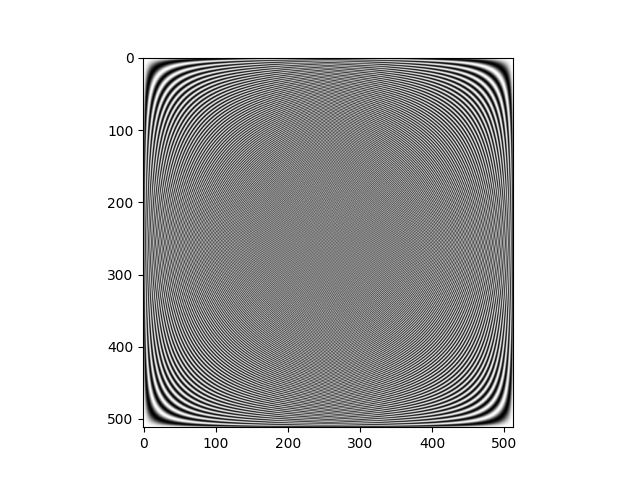
\includegraphics[width=\linewidth]{Figures/dft.png}
	  \caption{Square DFT.}
	  \label{fig:dft-square}
	\end{subfigure}
	\begin{subfigure}{.45\textwidth}
	  \centering
	  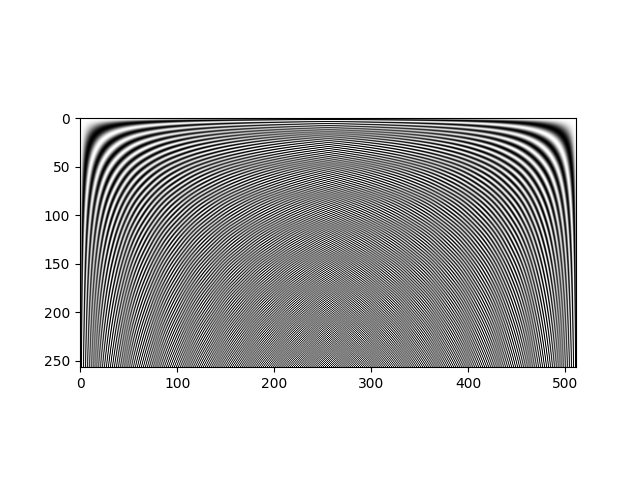
\includegraphics[width=\linewidth]{Figures/dft_non_square.png}
	  \caption{Non-square DFT.}
	  \label{fig:dft-non-square}
	\end{subfigure}
	\caption{Visual representations of the forward matrix operators.}
	\label{fig:dft}
\end{figure}

Now we need the inverse operator, which then needs to be $N$ by $N/2+1$.
If the assumption that the transpose matrix is the inverse operator holds, then building the inverse operator from the definition of the inverse Fourier transform should work.
The closest I have been able to come up with is the following definition:
\begin{align}
	&\omega = e^{2\pi i / N}\\
	&W^{r^{-1}}_{x_i \nu_i} = \frac{1}{N/2 +1} (\omega^{\nu_i x_i} - 1).
\end{align}

The matrix operators are shown in Figure \ref{fig:idft}.

\begin{figure}[ht]
	\centering
	\begin{subfigure}{.45\textwidth}
		\centering
		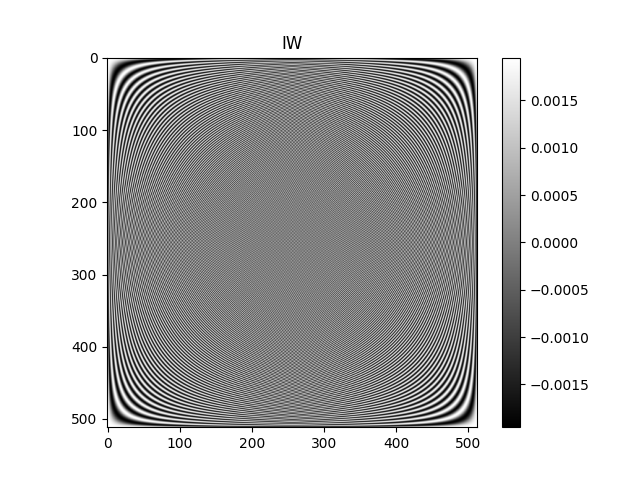
\includegraphics[width=\linewidth]{Figures/idft.png}
		\caption{Square inverse DFT.}
		\label{fig:idft-square}
	\end{subfigure}
	\begin{subfigure}{.45\textwidth}
		\centering
		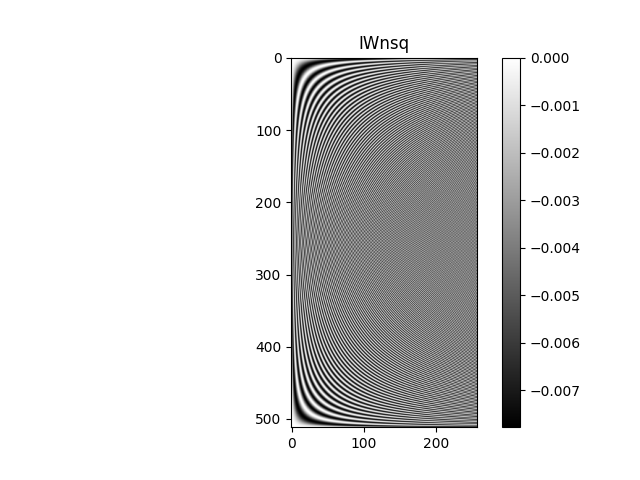
\includegraphics[width=\linewidth]{Figures/idft_non_square.png}
		\caption{Non-square inverse DFT.}
		\label{fig:idft-non-square}
	\end{subfigure}
	\caption{Visual representations of the inverse matrix operators.}
	\label{fig:idft}
\end{figure}

Nothing seems obviously wrong with the non-square version of the operator.
However, Figure \ref{fig:problems} shows what the matrix multiplication of the forward and inverse operators ($W^{r^{-1}}W^r$) looks like (which we expect to be the identity matrix) and the close-up of the difference between the original real-valued input and the output after putting it through our built non-square DFT and inverse DFT operators.

\begin{figure}[ht]
	\centering
	\begin{subfigure}{.45\textwidth}
	  \centering
	  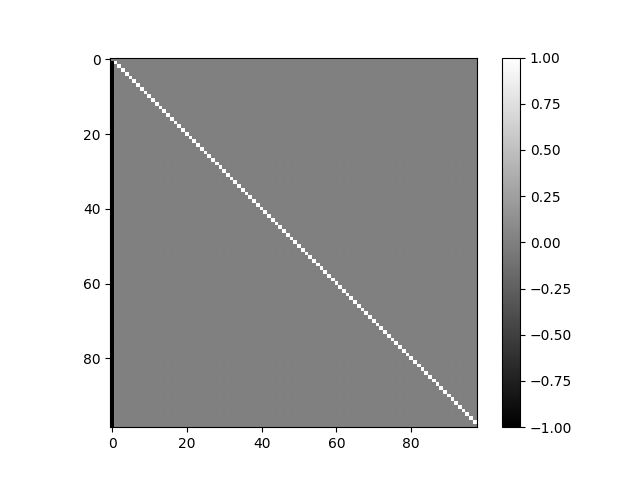
\includegraphics[width=\linewidth]{Figures/multiplied.png}
	  \caption{Multiplication of the forward and inverse operators.}
	  \label{fig:problems-multiplication}
	\end{subfigure}
	\begin{subfigure}{.45\textwidth}
	  \centering
	  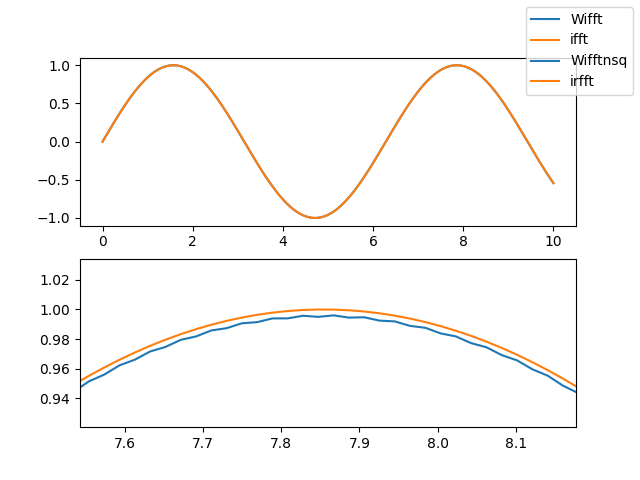
\includegraphics[width=\linewidth]{Figures/bumps.png}
	  \caption{Close-up of the difference between the original and the output.}
	  \label{fig:problems-closeup}
	\end{subfigure}
	\caption{Visual representations of the problems with the non-square inverse DFT.}
	\label{fig:problems}
\end{figure}

I also tried simply taking the hermitian conjugate of the DFT matrix instead of building the inverse DFT matrix "from scratch" and that seems to wield the same results.

\section{Mapmaking for FTS}

When looking at each individual interferogram (and therefore only looking at one pixel), there is a fairly simple matrix formulation of the maximum likelihood mapmaking equation, which which relates the spatial distance in the instrument $x$ with sky frequency $\nu$ and reads
\begin{equation}
	(F^T_{\nu; x} N^{-1}_{x;x} F_{x;\nu}) m_\nu = F^T_{\nu; x} N^{-1}_{x;x} d_x,
\end{equation}
where ; in the index separates the two dimensions of the matrix.

Now the standard mapmaking equation relates time $t$ with position in the sky $p$ and reads
\begin{equation}
	(P^T_{p;t} N^{-1}_{t;t} P_{t;p})m_p = P^T_{p;t} N^{-1}_{t;t}d_t.
\end{equation}

Now in order to be able to treat pixel correlations, we need to put the two together, which I think will look like this:
\begin{equation}
	(P^T_{\nu p;\nu}F^T_{\nu;xt} N^{-1}_{xt;xt} F_{xt;\nu}P_{\nu;\nu p})m_{\nu p} = P^T_{\nu p;\nu}F^T_{\nu;xt} N^{-1}_{xt;xt}d_{xt}.
\end{equation}

\subsection{Revised data model and corresponding ML mapmaking equation}

After speaking to Sigurd, he came up (somewhat independently) with the following data model:
\begin{equation}
	d_i = P_i F T_i m + n,
\end{equation}
where $i$ for the FIRAS case would correspond to temperature bins. And the corresponding ML mapmaking equation would then be:
\begin{equation}
	\hat m = \left(\sum_i T_i^T F^T P_i^T N^{-1} P_i F T \right)^{-1} \sum_i T_i^T F^T P^T N^{-1} d_i,
\end{equation}
where $F$ here should be cosine transforms.

We spoke about it after and mentioned that it actually might make more sense to add the ICAL (and others) back in when the data is in IFG space, which then even can ignore these temperature bins.
This would probably mean that we need to do all other low-level IFG processing before entering this "pipeline" too, like removing the transient reponse from the  onboard digital filters, etc.

\subsection{Mapmaking without taking into account frequency correlations}

For the sake of starting with something simple, we will assume that we have white noise and no frequency correlations (which is not true, the current noise estimate (without taking into account frequency correlations) for FIRAS is shown in Figure \ref{fig:noise-estimation}, which seems to be white + blue noise).

\begin{figure}[ht]
	\centering
	\begin{subfigure}{.45\textwidth}
	  \centering
	  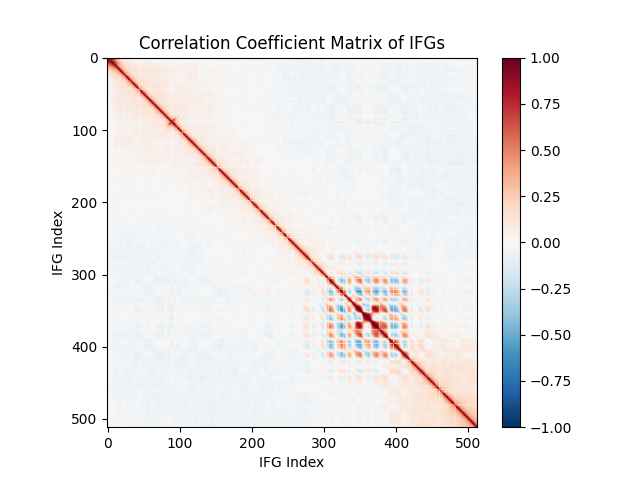
\includegraphics[width=\linewidth]{Figures/cov.png}
	  \caption{Noise covariance matrix not taking into account frequency correlations (size is 512 x 512). In order to subtract the signal to estimate this, I simply subtracted one IFG from the next and so on.}
	  \label{fig:cov-matrix}
	\end{subfigure}
	\begin{subfigure}{.45\textwidth}
	  \centering
	  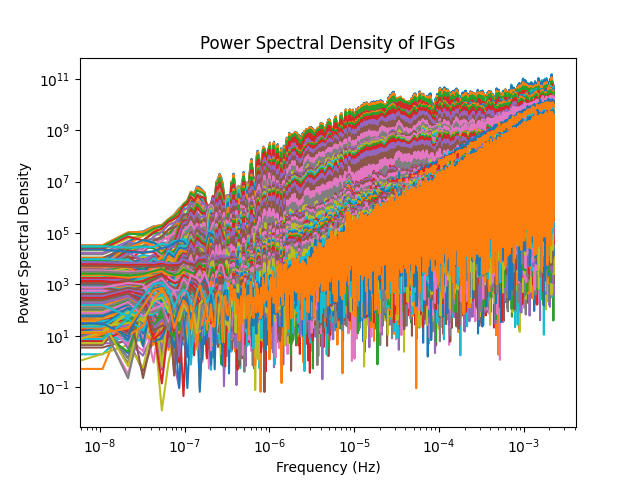
\includegraphics[width=\linewidth]{Figures/psd.png}
	  \caption{Noise PSD not taking into account frequency correlations (Fourier transform was made along NIFG). In order to subtract the signal to estimate this, I simply subtracted one IFG from the next and so on.}
	  \label{fig:psd}
	\end{subfigure}
	\caption{Noise estimations without taking into account frequency correlations.}
	\label{fig:noise-estimation}
\end{figure}

I now believe that there is no difference in where we place the (let's call it) space distance Fourier transform $F_x$ in relation to the pointing matrix in our data model, if we are considering a stop and stare approach (which we are for now), because it is the same to first bin and then take the Fourier transform or vice-versa. Taking this into account, the most efficient way to program is taking the Fourier transform of the following after binning:

\begin{equation}
	\hat m_p = \frac{\sum_{i \in p}\frac{d_i}{\sigma_i^2}}{\sum_{i \in p}\frac{1}{\sigma_i^2}}.
\end{equation}

For now we are also assuming an instrument that is not differential, i.e. there is no sutraction of an internal calibration because, even though FIRAS is differential, a general FTS does not need to be. In order to take this into account, the two options are to either consider a completely different equation and Fourier transform as the first step and then subtract in sky frequency space or to leave it as is and subtract in interferogram space.

\subsection{Dealing with beam movement while taking interferograms}

In FIRAS, and likely for any FTS, the instrument is still moving while taking interferograms (i.e. it does not stop and stare at a single pixel while it is taking one interferogram). In particular, FIRAS averages a number of interferograms onboard before sending them down. For example, for a short scan, the instrument takes one full interferogram, the MTM flys back, another interferogram is taken, the MTM flys back again, and so on, until 16 full interferograms are taken, with a full cycle, for example while taking data in the slow mode (0.8 cm/s velocity of the MTM), taking 55.36 seconds in total. As such, 16 onboard interferograms correspond to 1 interferogram in our data ("telemetered" interferograms), when taking data in the short mode. Timing info is given in \url{https://lambda.gsfc.nasa.gov/data/cobe/firas/ancil/FIRAS_FEX_MTMSWEEP.TXT}.

As such, we want to understand, for each telemetered interferogram and their latitude and longitude coordinates, how many and which pixels they correspond to, and how much data is taken corresponding to that pixel. For example, if one telemetered interferogram was taken equally over two pixels, the part of the pointing matrix corresponding to this goes from
\begin{equation}
	P = \begin{pmatrix}
		0 & 1 \\
		0 & 0
	\end{pmatrix}
\end{equation}
to
\begin{equation}
	P = \begin{pmatrix}
		0.5 & 0.5 \\
		0 & 0
	\end{pmatrix}.
\end{equation}

We also know that the pointing solution for each interferogram is given in the middle of taking each telemetered interferogram. (Section 4.2 of the explanatory supplement) The FIRAS line of sight traces a path along a line of approximately constant ecliptic longitude. The beam is of 7 degrees. The beam moves at 3.5 degrees per minute. 

%-------------------------------------------------------------
%                                       Table with references 
%-------------------------------------------------------------
%

\bibliographystyle{aa}
\bibliography{../../common/CG_bibliography,../../common/Planck_bib}
\end{document}
%%%% End of aa.dem
